\documentclass[tikz,border=2pt]{standalone}
\usepackage{amsmath,amssymb}
\usepackage{tikz}

\begin{document}
% Stars and bars: distributing 6 identical items into 3 boxes is the same as arranging
% 6 stars and 2 bars in a row; the pattern **|*|*** means (2, 1, 3).
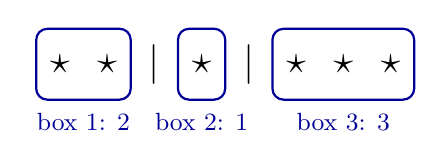
\begin{tikzpicture}[every node/.style={font=\small}]
	\foreach \x/\s in {0/$\star$, 0.6/$\star$, 1.2/$|$, 1.8/$\star$, 2.4/$|$, 3.0/$\star$, 3.6/$\star$, 4.2/$\star$} {
		\node[font=\Large] at (\x,0) {\s};
	}
	\draw[blue!60!black, thick, rounded corners=4pt] (-0.3,-0.45) rectangle (0.9,0.45);
	\draw[blue!60!black, thick, rounded corners=4pt] (1.5,-0.45) rectangle (2.1,0.45);
	\draw[blue!60!black, thick, rounded corners=4pt] (2.7,-0.45) rectangle (4.5,0.45);
	\node[blue!60!black, anchor=north] at (0.3,-0.5) {box 1: $2$};
	\node[blue!60!black, anchor=north] at (1.8,-0.5) {box 2: $1$};
	\node[blue!60!black, anchor=north] at (3.6,-0.5) {box 3: $3$};
\end{tikzpicture}
\end{document}
